\chapter{Stand der Technik und verwandte Arbeiten}
\label{ch:03_acedemic_and_industry_state}

Dieses Kapitel analysiert den aktuellen Forschungsstand zu Forward- und Deferred-Ren\-der\-ing\--Ar\-chi\-tek\-tu\-ren
sowie moderne Industriepraktiken im Bereich hybrider Architekturen und selektiver Stilisierung.
Durch die Betrachtung bestehender Verfahren im Kontext des \ac{NPR} werden deren konzeptionelle und leistungstechnische
Limitierungen aufgezeigt.
Die Identifikation dieser Schwachstellen sowie der Mangel an empirischen Vergleichsdaten dienen der Bestimmung der
zugrundeliegenden Forschungslücke, begründen die in dieser Arbeit durchgeführte holistische Systemanalyse und
ermöglichen die wissenschaftliche Einordnung des entwickelten Evaluations-Frameworks.


\section{Klassische Rendering-Architekturen und deren Implikationen für das NPR}
\label{sec:0301_academic_state}

% Einleitung.
Deferred-Rendering-Paradigmen stellen sowohl in der akademischen Forschung als auch in der industriellen Praxis
etablierte Standards dar~\cite[S.~2]{mallettDeferredAdaptiveCompute2018}.
Moderne Echtzeit-Rendering-Pipelines werden maßgeblich von komplexen Beleuchtungsanforderungen getrieben, wodurch das
effiziente Handhaben von Deferred-Architekturen in den Fokus rückt.
Gleichzeitig werden im Bereich des Forward-Renderings durch diverse Optimierungsverfahren die klassischen Schwächen
dieses Ansatzes zunehmend relativiert~\cite{olssonClusteredDeferredForward2012, haradaForwardBringingDeferred2012}.
Die Wahl des Rendering-Ansatzes richtet sich somit in der Praxis streng nach den spezifischen Leistungs- und
Qualitätsanforderungen der jeweiligen Anwendung.
Der wissenschaftliche Diskurs untersucht diesbezüglich Lösungen in Bezug auf Leistungsfähigkeit und Grenzen beider
Grundarchitekturen.

% Forward Rendering.
Der primäre architektonische Nachteil klassischer Forward-Rendering-Ansätze liegt, wie in
Kapitel~\ref{subsec:020201_forward_rendering} dargelegt, im multiplikativen Aufwand von
$\mathcal{O}(N_{\text{obj}} \cdot N_{\text{light}})$ bei hoher
Geometrie- und Beleuchtungskomplexität.
Zusätzlich zu dieser Komplexität ergibt sich eine kombinatorische Zunahme der Shader-Permutationen (spezifisch
kompilierte Shader-Varianten für jeweilige Material- und Lichtkonfigurationen), sobald diverse Materialeigenschaften
und Lichttypen in einer Szene verrechnet werden müssen.
Dieser Limitierung liegt die inhärente Eigenschaft von Forward-Pipelines zugrunde, bei hoher Szenen-Entropie
zwangsweise eine gewisse Menge an Overdraw zu erzeugen~\cite[S.~1]{fatahalianReducingShadingGPUs2010}.
Ansätze wie ein Z-Prepass zur frühzeitigen Verwerfung verdeckter Fragmente gehören in Forward-Pipelines zwar zum
Standard~\cite[S.~57]{burnsVisibilityBufferCacheFriendly2013}, reichen bei hoher Objekt- und Lichtkomplexität
jedoch nicht aus, um die Effizienz von Deferred-Ansätzen zu
erreichen~\cite[S.~4]{Thaler2011DeferredRendering}.
Modernere Techniken wie \textit{Clustered Forward} oder \textit{Forward+} adressieren dieses Problem, indem
Lichtquellen in 2D-Kacheln oder 3D-Clustern räumlich sortiert
werden~\cites{olssonClusteredDeferredForward2012, haradaForwardBringingDeferred2012}.
Dies ermöglicht eine Effizienz, die Deferred-Ansätzen nahekommt, während der primäre Vorteil der Forward-Architektur,
die hohe Flexibilität bei der Materialauswertung, erhalten bleibt.

% Deferred Rendering.
Deferred-Rendering-Pipelines haben sich in Umgebungen mit hoher geometrischer Komplexität und anspruchsvollen
Beleuchtungsszenarien weitestgehend durchgesetzt~\cite[Abschn.~2]{mallettDeferredAdaptiveCompute2018}, weisen jedoch
ebenfalls diverse architektonische Limitierungen auf.
Der signifikanteste Flaschenhals ist die hohe Auslastung der Speicherbandbreite (Memory Bandwidth), welche durch den
permanenten Schreib- und Lesezugriff auf den \ac{G-Buffer} induziert
wird~\cite[S.~55]{burnsVisibilityBufferCacheFriendly2013}.
Ein moderner Lösungsansatz aus der Forschung ist die Implementierung entkoppelter Architekturen wie des
\ac{V-Buffer}~\cite{burnsVisibilityBufferCacheFriendly2013}, welcher als Shading-Grundlage für hochkomplexe
Geometrie-Pipelines wie der \textit{Nanite}-Architektur in der Unreal Engine 5
dient~\cite[Folie~\textit{Visibility Buffer}]{Karis_Nanite_SIGGRAPH_Advances_2021_final}.
Im Gegensatz zum traditionellen \ac{G-Buffer} speichert der V-Buffer pro Pixel lediglich minimale geometrische Metadaten
(wie Primitive- und Instanz-IDs) sowie Tiefenwerte.
Die speicherintensive Materialauswertung wird vollständig in einen nachgelagerten Pass verschoben.
Neben der Bandbreitenproblematik existieren in klassischen Deferred-Architekturen zwei weitere praktische Nachteile:
die fehlende native Kompatibilität mit hardwarebasiertem \ac{MSAA} sowie eine grundlegende Einschränkung bei
transluzenten Oberflächen.
\ac{MSAA} glättet Objektkanten bereits während des geometrischen Rasterisierungsschritts (vgl.\ Kap.~\ref{0202}).
Da Deferred Rendering die Beleuchtung jedoch erst im nachgelagerten Bildraum berechnet, stehen diese Geometriedetails
der Kanten nicht mehr zur Verfügung.
Für Kantenglättung in Deferred-Pipelines werden temporale Verfahren wie \ac{TAA} verwendet, die dieses Problem lösen,
indem sie das fertige Bild über mehrere Frames hinweg zeitlich
verrechnen~\cites[S.~5]{Thaler2011DeferredRendering}{taaantialiasing}.
Die Evaluierung semitransparenter Geometrie ist im reinen Deferred-Pfad nicht lösbar, da ein Standard-\ac{G-Buffer}
pro Pixel nur eine einzige diskrete Tiefenschicht speichert.
Da für transparentes Alpha-Blending jedoch die Material- und Lichtwerte mehrerer hintereinander liegender Flächen
entlang der Sichtachse verrechnet werden müssen, gehen die erforderlichen Informationen verdeckter Schichten verloren.
Dieses Defizit wird in der industriellen Praxis standardmäßig über einen nachgelagerten Forward-Pass für
transluzente Objekte gelöst~\cite[S.~56]{burnsVisibilityBufferCacheFriendly2013}.

% Non-Photorealistic-Rendering.
Hinsichtlich des \ac{NPR} unterscheidet die aktuelle Literatur primär zwischen
\textit{Object-Space}- und
\textit{Screen-Space}-Methoden~\cite[S.~148]{magdicsPostprocessingNPREffects2013}.
Object-Space-Ansätze sind in der Regel in Forward-Pipelines verankert und berechnen Stilisierungen direkt auf
der Geometrie, was eine granulare, objektbasierte Anpassung ermöglicht.
Bei hoher Szenenkomplexität weisen diese Verfahren jedoch eine unzureichende Skalierbarkeit auf, was primär auf den
Fragment-Overdraw bei rechenintensiven Abstraktionseffekten zurückzuführen
ist~\cite[S.~1]{fatahalianReducingShadingGPUs2010}.
Die moderne Rendering-Forschung weicht zur Umgehung dieser Performance-Limits oft auf Screen-Space-Methoden
(Post-Processing) aus, was architektonisch stark den Paradigmen des Deferred-Renderings entspricht.
Wie~\textcite[S.~148]{magdicsPostprocessingNPREffects2013} beschreiben, ist diese Screen-Space-Verarbeitung zwar
sehr effizient, löst jedoch den direkten Bezug zum individuellen 3D-Objekt auf, wodurch etwa die selektive Stilisierung
in der praktischen Umsetzung erschwert wird.
Die Nutzung von Deferred-Rendering-Architekturen ermöglicht die Rekonstruktion des räumlichen Kontextes im
Post-Processing.
Wie~\textcite[Abschn.~3.2]{Thaler2011DeferredRendering} anmerkt, basiert die Lösung dieses Problems auf einem
zweistufigen Ansatz: Im ersten Schritt werden alle räumlichen 3D-Informationen (Tiefen, Normalen) im \ac{G-Buffer}
gesammelt, um diese Metadaten im zweiten Schritt für globale, Screen-Space-basierte \ac{NPR}-Effekte nutzbar zu machen.
Dies ermöglicht es, Stilisierungen im Screen-Space auch geometriebewusst durchzuführen.
Klassische Deferred-Pipelines weisen in diesem Kontext jedoch eine fundamentale Schwäche bezüglich der Materialvielfalt
auf~\cite[S.~1]{haradaForwardBringingDeferred2012}.
Das Auswerten zahlreicher spezifischer Stilisierungen in einem vereinheitlichten Screen-Space-Pass
führt zu starken Performance-Einbußen, da abweichende Materialpfade benachbarter Pixel innerhalb eines Warps
zu der in Kapitel~\ref{subsec:020303_warp_divergence_and_register_pressure} beschriebenen Warp-Divergence
führen~\cite[Abschn.~2.6]{Thaler2011DeferredRendering}.
In der Konsequenz bleiben performante Stilisierungen bei klassischem Deferred-Rendering meist auf globale
Post-Processing-Filter beschränkt~\cite[S.~148]{magdicsPostprocessingNPREffects2013}.

% Fazit.
Zusammenfassend lässt sich festhalten, dass reine Forward- oder Deferred-Architekturen in modernen Produktionen
selten in ihrer Reinform existieren, da die Forschung im Bereich der Rendering-Architekturen primär auf
hybride Lösungsansätze, im Sinne einer Kombination verschiedener Pipeline-Paradigmen, sowie die Reduktion
architektonischer Engpässe fokussiert ist~\cite[S.~56]{burnsVisibilityBufferCacheFriendly2013}.
Obwohl die Literatur diverse architektonische Lösungen für hohe Geometrie- und Beleuchtungskomplexität bietet,
unterliegt die spezifische Schnittmenge von Deferred-Pipelines und selektivem \ac{NPR} weiterhin
praktischen und Performance-technischen Limitierungen.
Die Analyse der angewandten Industriepraxis sowie der Architektur moderner Game-Engines zeigt auf, wie
diese Hürden in der Praxis umgangen werden.


\section{Rendering-Pipelines und Stilisierung in der Industriepraxis}
\label{sec:0302_industry_state}

% Einleitung: Konflikt.
Der theoretische Konflikt zwischen der für Deferred Shading charakteristischen Homogenität des Beleuchtungspasses und
der für \ac{NPR} oft erforderlichen Heterogenität individueller Stilisierungen zwingt die
Industrie zu architektonischen Kompromissen.
Der Ansatz, alle für komplexe \ac{NPR}-Modelle benötigten Parameter separat in den \ac{G-Buffer} zu schreiben, führt
unweigerlich zu einem sogenannten \textit{Fat \ac{G-Buffer}}~\cite[S.~71]{AdvancesRealTimeRendering}.
In modernen AAA-Produktionen der Spieleindustrie werden teilweise bis zu acht \acp{RT} gleichzeitig
beschrieben, was starke Bandbreiten-Engpässe (Memory Bandwidth Bottlenecks) verursachen
kann~\cite[S.~884]{akenine-mollerRealtimeRendering2019}.
Folglich existiert in der Industriepraxis kein universeller beziehungsweise einheitlicher Deferred-\ac{NPR}-Algorithmus.
Stattdessen greifen Entwickler auf hoch spezialisierte, kompromissbehaftete Architekturen zurück, um selektive
Stilisierungen innerhalb gegebener Hardware-Grenzen zu realisieren.

% Ansatz A: G-Buffer Packing.

\paragraph{G-Buffer Packing}
Ein primärer Lösungsansatz hierfür ist das \textit{\ac{G-Buffer} Packing} in Kombination mit
\enquote{Shading-Model-IDs}.
Die Wiederverwendung oder Neudefinition von Datenkanälen, die für das klassische \ac{PBR} vorgesehen sind,
reduziert den Bedarf an Speicherbandbreite.
Ein exemplarisches Vorgehen zeigt das auf Toon-Rendering fokussierte Spiel \textit{Hi-Fi RUSH}: Hierbei werden regulär
für \ac{PBR}-Daten vorgesehene \ac{G-Buffer}-Kanäle gezielt umgewidmet, um diese stattdessen mit spezifischen \ac{NPR}-Parametern und
ID-Masken zu belegen (siehe Abbildung~\ref{fig:g-buffer_hifirush}).
Ein ähnliches Verfahren zeigt die Architektur von \textit{Uncharted 4}, in der eine komprimierte \textquote{Material-ID} im
\ac{G-Buffer} mitgeführt wird, um im nachgelagerten Lighting-Pass zwischen verschiedenen Shader-Features zu
differenzieren~\cite[Folie~\enquote{Deferred Pipeline}]{deferredLightinginUncharted4}.
Überträgt man diesen Ansatz auf das \ac{NPR}, um eine selektive Stilisierung direkt im regulären Lighting-Pass zu verankern,
führt dies in der Praxis unweigerlich zu monolithischen
Shader-Strukturen (Uber-Shadern)~\cite[Folie~\enquote{Problems}]{deferredLightinginUncharted4}.
Eine steigende Stil- und Materialvielfalt induziert innerhalb eines solchen Shaders einen massiven Registerdruck
(\textit{Register Pressure}) und provoziert durch die notwendigen Fallunterscheidungen zeitgleich ineffiziente
\textit{Warp Divergence} (vgl.\ Kap.~\ref{subsec:020303_warp_divergence_and_register_pressure}).
Diese architektonischen Flaschenhälse limitieren die
Gesamteffizienz der Rendering-Pipeline bei hoher Szenen-Entropie auf der \ac{GPU}
signifikant~\cite[Abschn.~6]{schiedDeferredAttributeInterpolation2015}.

\begin{figure}[htbp]
    \centering
    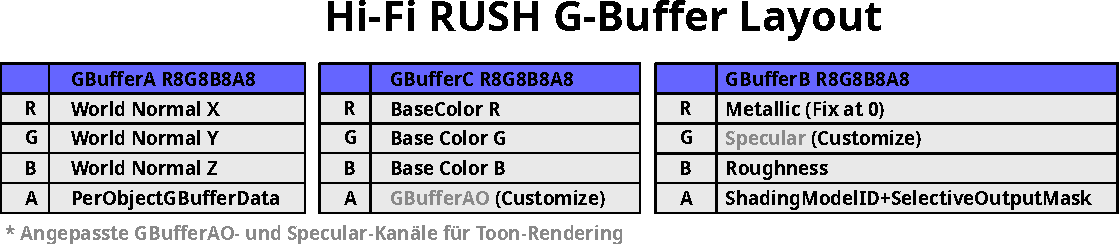
\includegraphics[width=0.95\textwidth]{abbildungen/hifirushgbuffer}
    \caption[Speicherlayout der Hi-Fi Rush G-Buffer]
    {Speicherlayout der Hi-Fi Rush G-Buffer. Eigene Darstellung in Anlehnung
    an \cite[Folie~\enquote{Our G-Buffer Layout}]{gameworksToonRenderingHiFi}.}
    \label{fig:g-buffer_hifirush}
\end{figure}

% Ansatz B: Hybrid Rendering.

\paragraph{Kombinierte Pipeline-Architekturen}
Moderne Engines implementieren hybride Architekturen, im Sinne einer Kombination verschiedener Pipeline-Paradigmen,
die eine grundlegende Deferred-Pipeline um einen nachgelagerten Forward-Pass erweitern, um den strukturellen
Limitierungen des \ac{G-Buffer}s hinsichtlich der Materialvielfalt zu begegnen.
Shading-Operationen, die hochkomplexe Materialbrechungen oder Transparenzen erfordern, werden in einem oder mehreren, an
den Deferred-Pass anschließenden, Forward-Rendering-Schritten berechnet und im finalen Framebuffer
kombiniert~\cite[S.~887]{akenine-mollerRealtimeRendering2019}.
Da dieser Forward-Pass jedoch die ursprünglichen Schwächen bezüglich der Beleuchtungskomplexität erbt, haben sich
Techniken wie \textit{Clustered Forward}~\cite{olssonClusteredDeferredForward2012} und
\textit{Forward+}~\cite{haradaForwardBringingDeferred2012} für diesen Hybridschritt etabliert.
Durch räumliches Frustum- oder Tile-basiertes \textit{Light-Culling} reduzieren sie die Anzahl der pro Fragment zu
berechnenden Lichtquellen drastisch.
Die Etablierung dieser Ansätze als Industriestandard zeigt sich beispielhaft an der \textit{id Tech 6} Engine:
Die Architektur kombiniert Clustered Deferred Shading für opake Basisgeometrie mit einem nachgelagerten
Clustered-Forward-Pass für transluzente Objekte und komplexe Effekte.
Durch die räumliche 3D-Cluster-Zuweisung bleibt die Lichtauswertung sowohl im Deferred- als auch im Forward-Pfad
performant~\cite{DOOM}.

% Ansatz C: Selektives Post-Processing.

\paragraph{Selektives Post-Processing}
Eine weitere gängige Industriepraxis bildet das selektive Screen-Space Post-Processing.
Hierbei wird die Stilisierung nicht auf Materialebene berechnet, sondern als bildbasierter 2D-Filter
in der Nachbearbeitung angebracht~\cite[S.~661]{akenine-mollerRealtimeRendering2019}.
Die Industrie implementiert Verfahren wie das \textit{Stencil-Masking}, um bei globalen Filtern dennoch eine selektive,
objektbasierte Zuweisung zu gewährleisten~\cite[S.~81]{AdvancesRealTimeRendering}.
In klassischen Deferred-Pipelines ist der \textit{Stencil-Buffer} (\textit{Schablonenspeicher}) hardwareseitig meist
direkt an den \textit{Depth-Buffer} (\textit{Tiefenpuffer}).
gekoppelt~\cite[Folie~\enquote{\ac{G-Buffer}: Our approach}]{valientDeferredRenderingKillzone}.
Anstatt Identifikationsnummern aufwendig als Farbinformationen in den regulären \ac{G-Buffer} zu schreiben, markieren die zu
stilisierenden Objekte ihre Pixel während des ersten Render-Durchlaufs (Geometrie-Pass) mit einem spezifischen
Referenzwert direkt im Stencil-Buffer.
Wird im Anschluss der Post-Processing-Filter über das fertige Bild gelegt, fungiert dieser Stencil-Wert als
Filterkriterium.
Die Grafikkarte prüft durch einen fest integrierten Hardware-Test, ob das aktuell berechnete Pixel zu einem markierten
Objekt gehört.
Ist dies nicht der Fall, wird das Fragment sofort verworfen.
Der Shader-Code für den Post-Processing-Effekt kommt somit nur genau dort zur Ausführung, wo er auch tatsächlich
benötigt wird.
Die \textit{CryEngine 3} demonstriert diese Praxis anschaulich: Sie nutzt \textit{Stencil-Masking} gezielt, um
rechenintensive Post-Processing-Algorithmen wie die Kantenerkennung (Edge-Detection) performant nur auf bestimmte
Objekte im Vordergrund anzuwenden, während der Rest der Szene unberührt
bleibt~\cite[S.~81]{AdvancesRealTimeRendering}.

% Zusammenfassung & Überleitung zum Gap.
Die Betrachtung der Industriepraxis offenbart, dass die Umsetzung selektiver, objektbasierter Stilisierungen in
Echtzeit-Engines gegenwärtig aus einem hochkomplexen Gefüge aus \ac{G-Buffer}-Manipulation, Uber-Shader-Branching und
hybriden Forward-Overlays besteht.
Dass moderne Rendering-Pipelines hierbei zunehmend fragmentieren, veranschaulicht die Analyse der aktuellen
AAA-Produktion \textit{PRAGMATA} (2026), deren selektives Post-Processing durch die Aufspaltung in zahlreiche isolierte
Render-Pässe und eigens generierte Masken realisiert
wird~\cite[Abschn.~\enquote{Frame}]{muhammadPrettyFramesPRAGMATA2026}
(vgl.\ Abbildung~\ref{fig:pragmata_pipeline_analysis}).
Solche architektonischen Kompromisse sind zwar für spezifische, isolierte Anwendungsfälle praktikabel, lassen sich
aber nur schwer auf Szenen mit extrem hoher Material- und Stil-Entropie unter Verwendung weniger leistungsfähiger
Hardware skalieren.
Aus dieser Diskrepanz zwischen hoch-spezialisierten Industrie-Workarounds und der Notwendigkeit einer skalierbaren
Lösung ergibt sich die Forschungslücke der vorliegenden Arbeit, welche im folgenden systematisch eingegrenzt wird.

%% PRAGMATA 1
%\begin{figure}[b]
%    \centering
%    \begin{subfigure}[b]{0.75\textwidth}
%        \centering
%        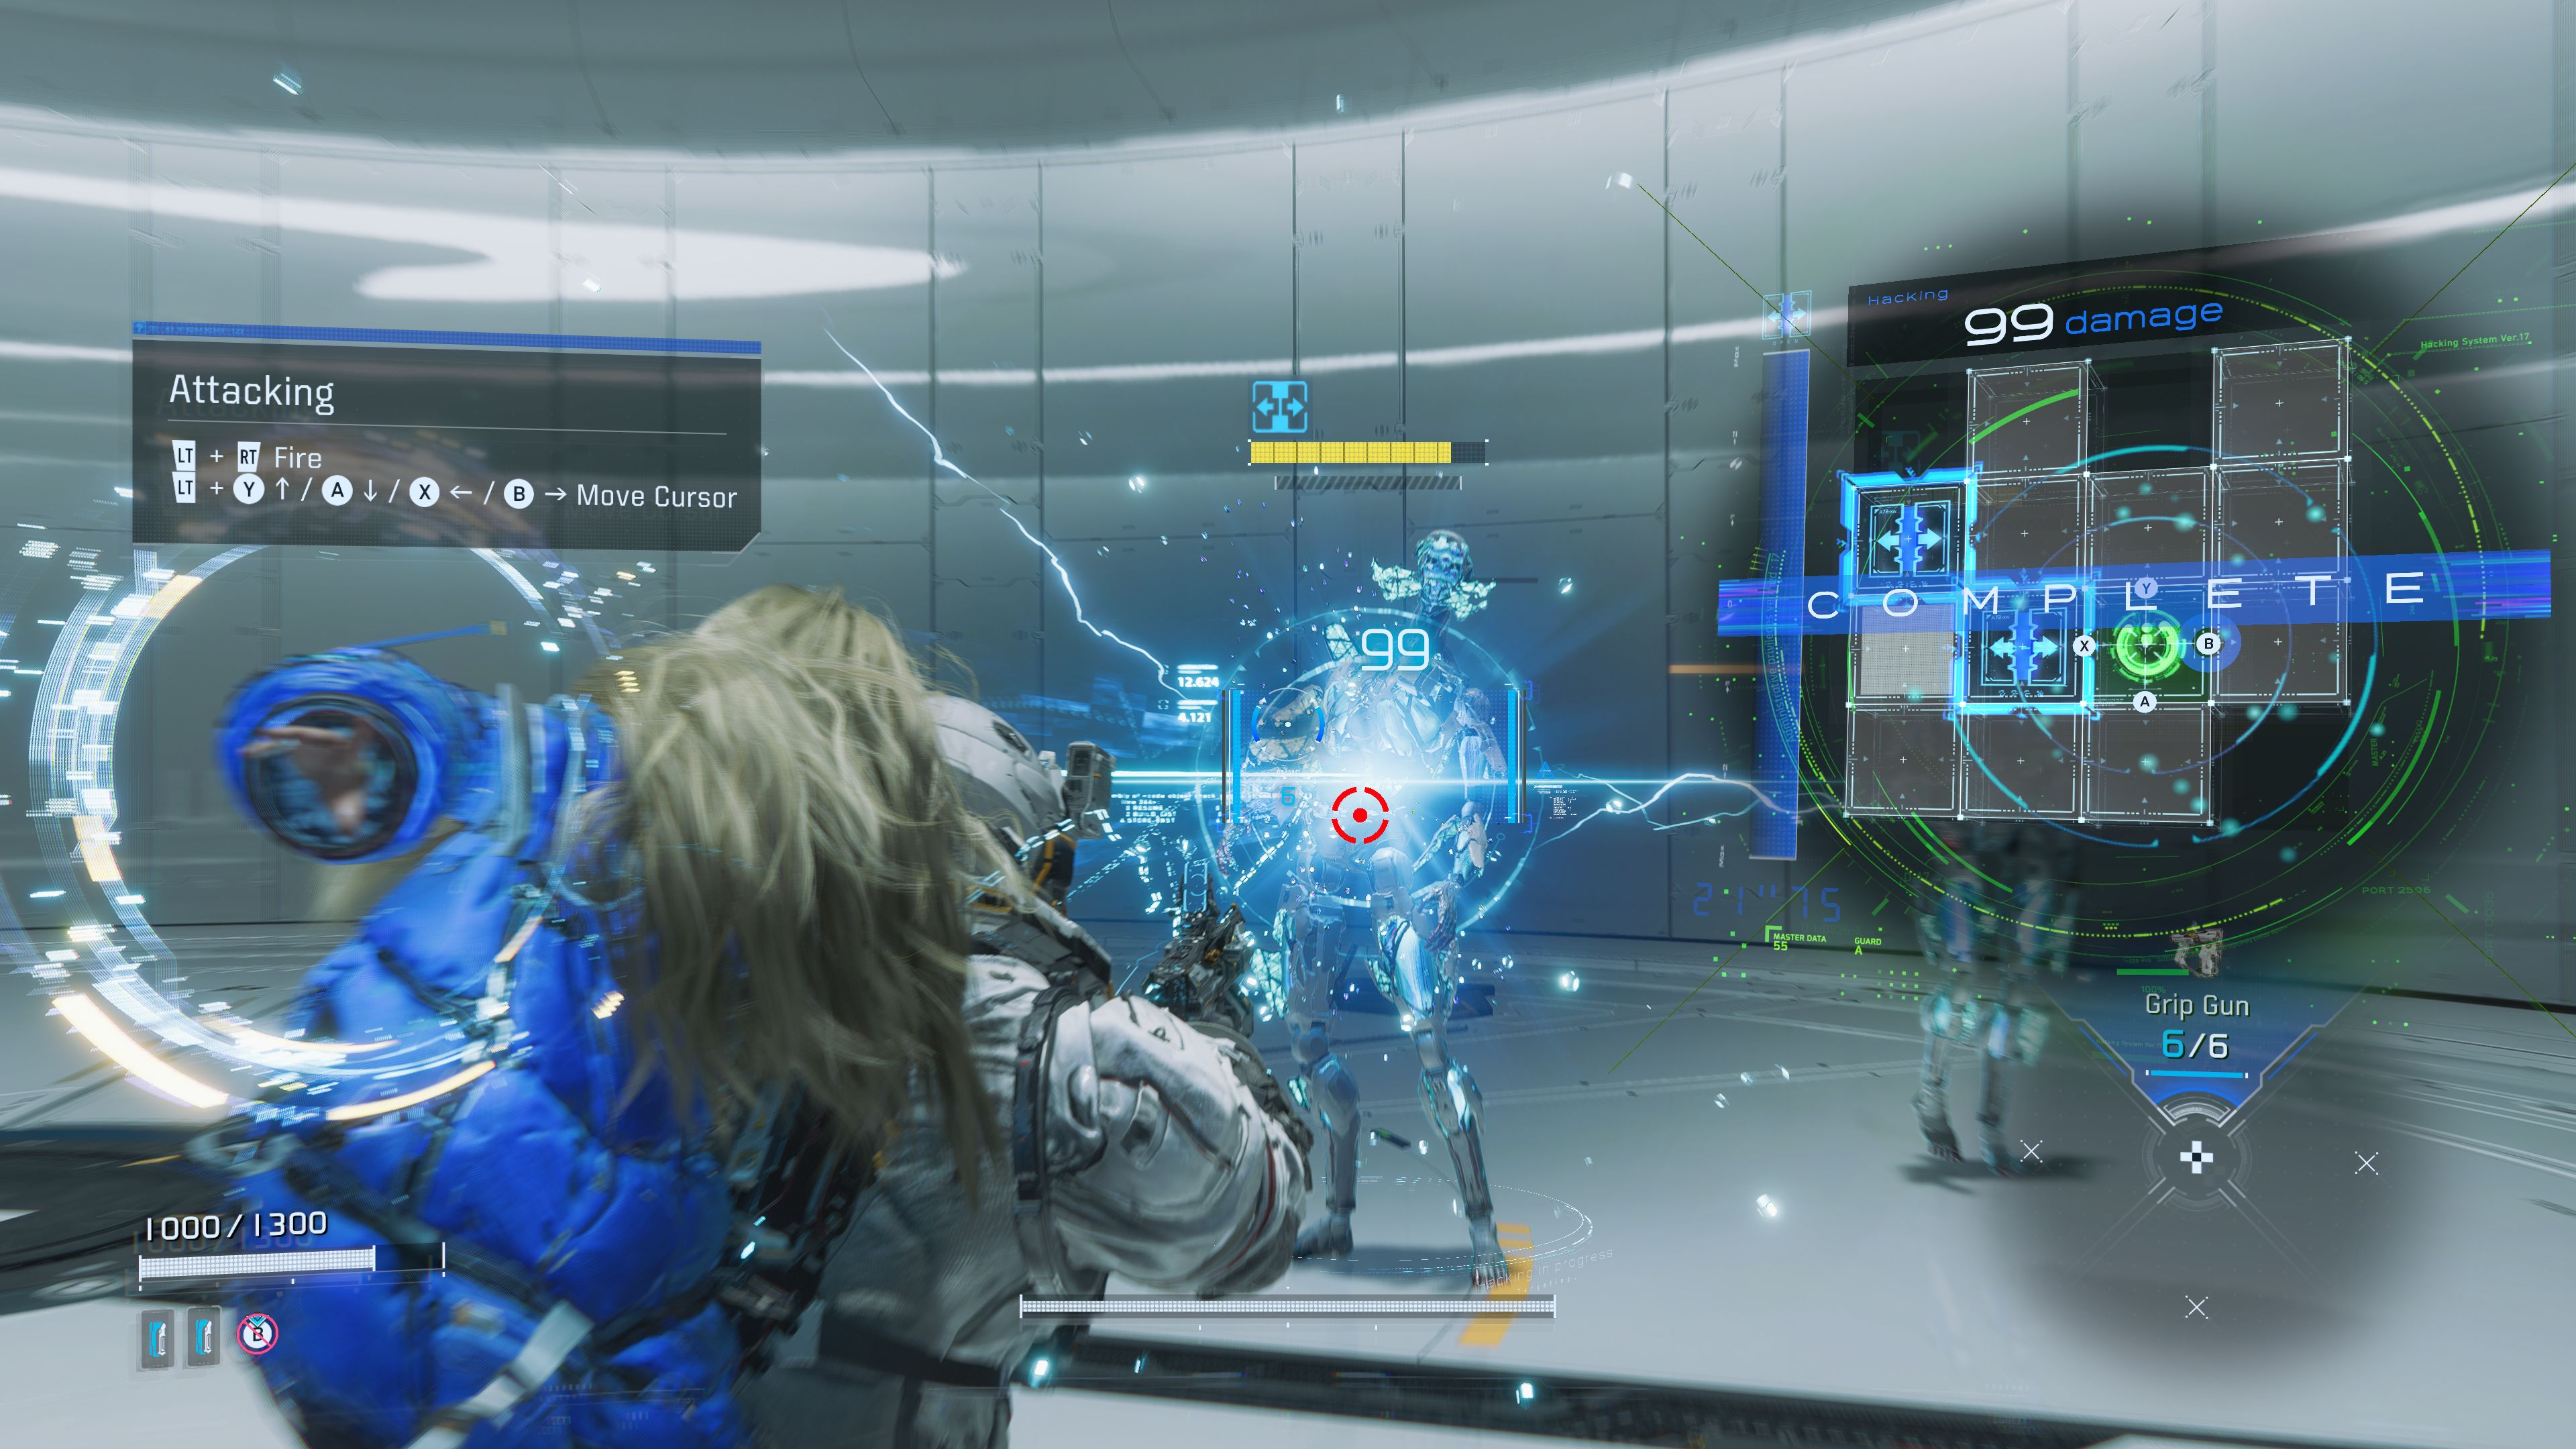
\includegraphics[width=\linewidth]{abbildungen/pragmata_screenshot}
%        \caption{Finales Rendering einer Spielszene.}
%        \label{fig:pragmata_final}
%    \end{subfigure}
%    \caption[Visualisierung der Pipeline-Fragmentierung in \textit{PRAGMATA}]{Visualisierung der Pipeline-Fragmentierung in modernen AAA-Produktionen am Beispiel von \textit{PRAGMATA}
%    (2026) zur Veranschaulichung spezialisierter Industrie-Workarounds~\cite{muhammadPrettyFramesPRAGMATA2026}.}
%    \label{fig:pragmata_pipeline_analysis}
%\end{figure}
%
%% PRAGMATA 2
%\begin{figure}[t]
%    \ContinuedFloat
%    \centering
%    \begin{subfigure}[b]{0.75\textwidth}
%        \centering
%        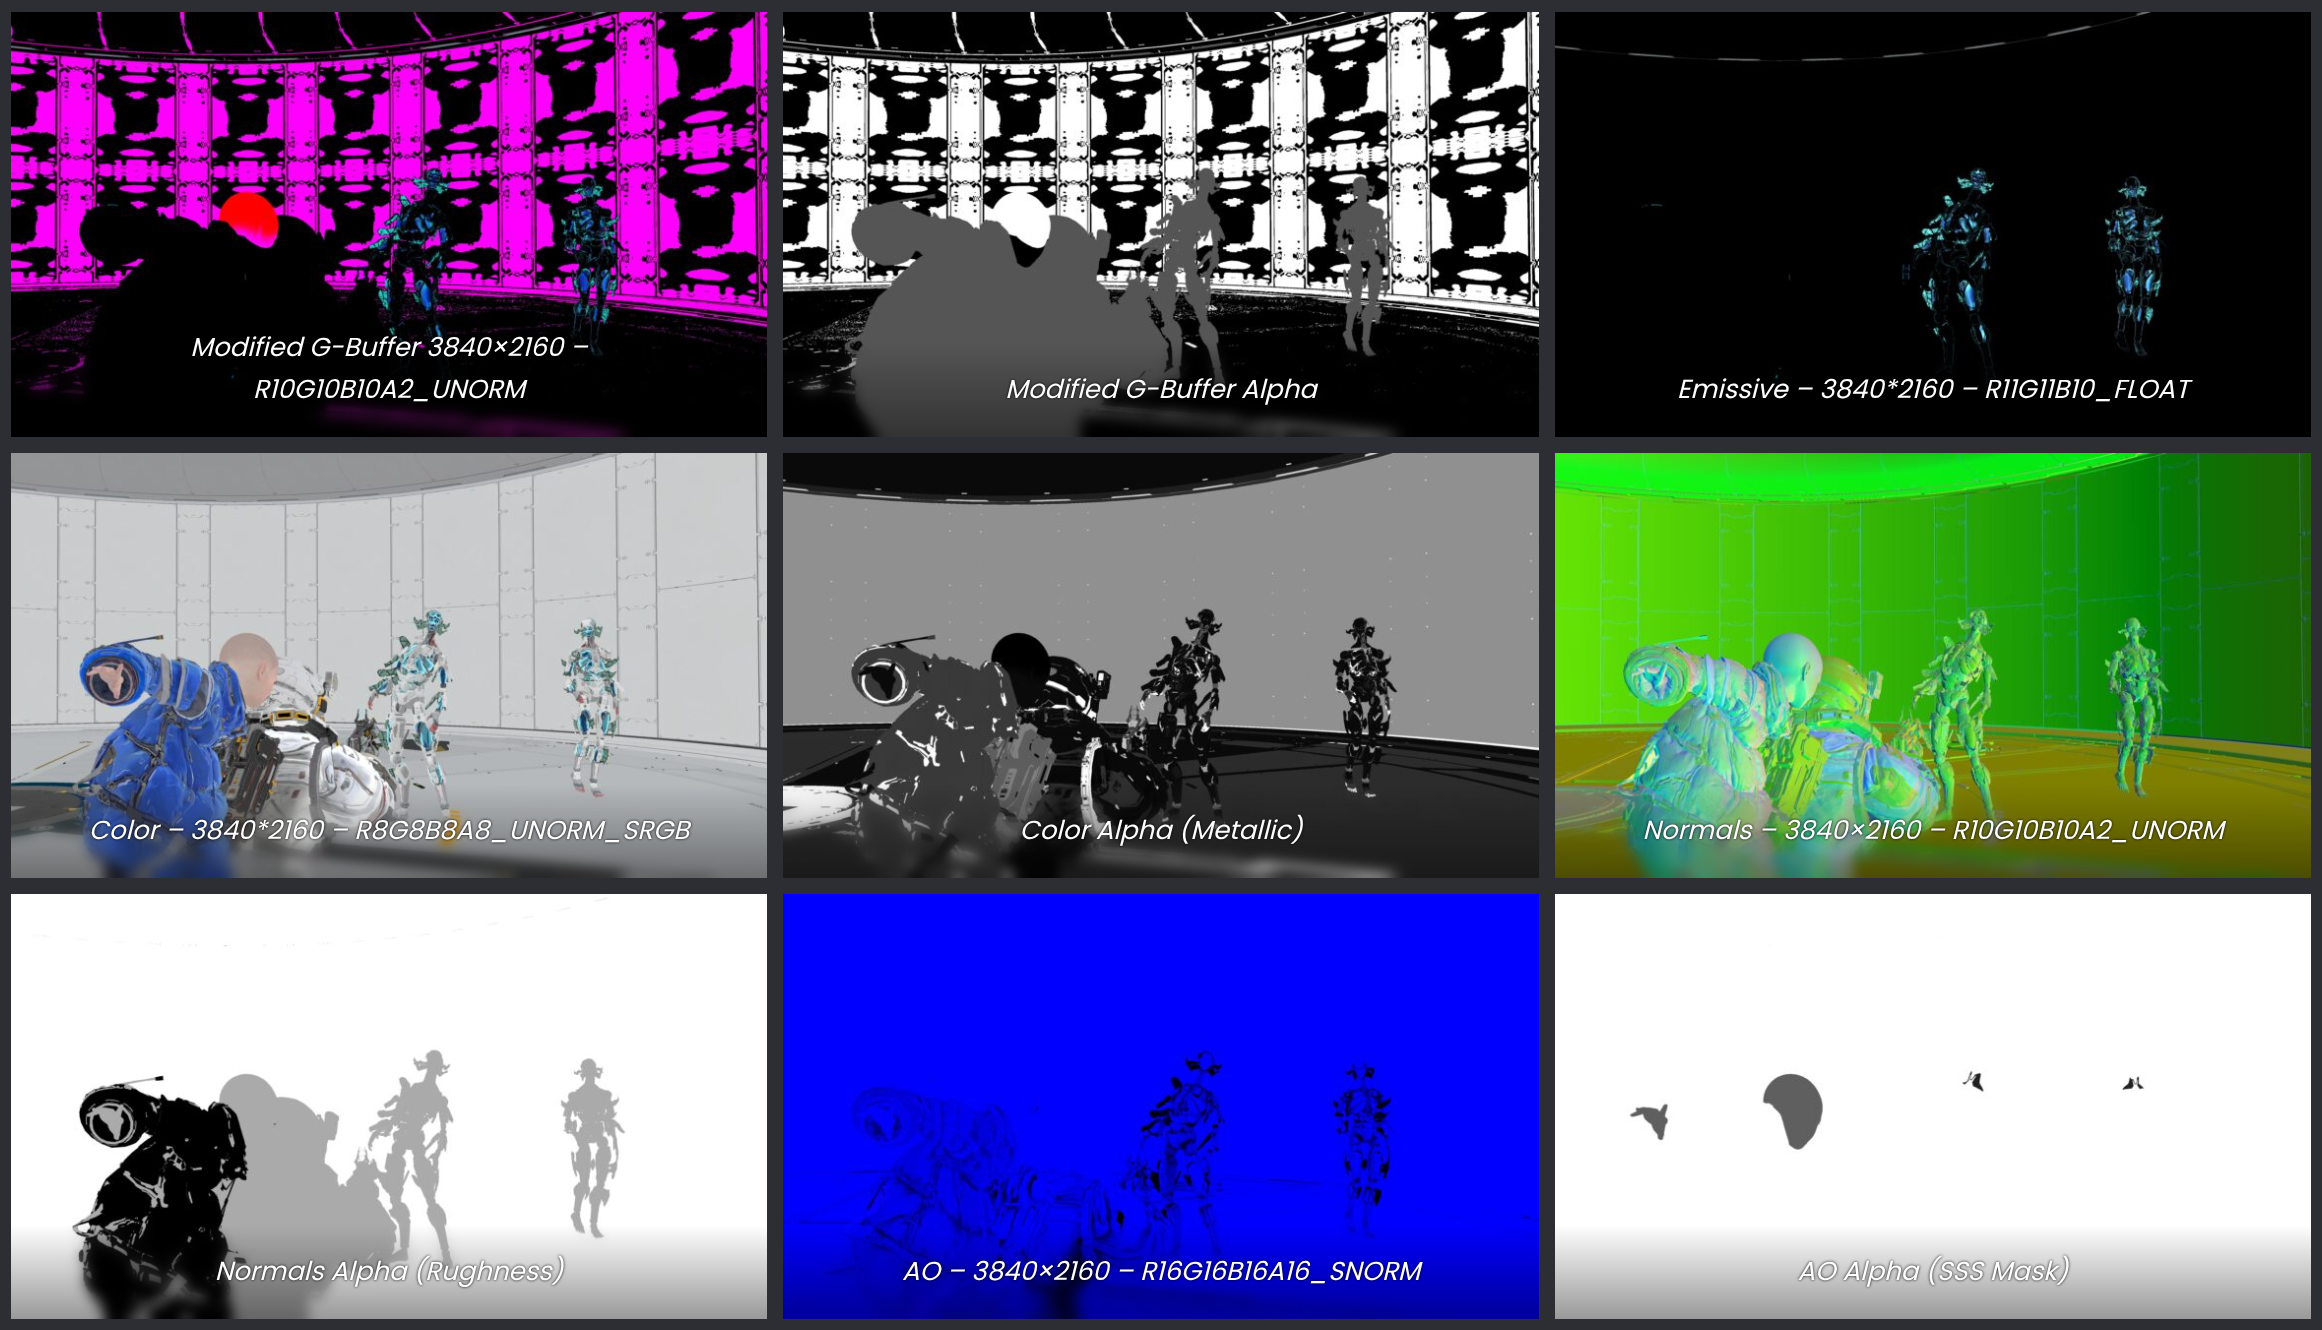
\includegraphics[width=\linewidth]{abbildungen/pragmata_gbuffer}
%        \caption{Frame-Analyse des korrespondierenden G-Buffers und der isolierten Render-Pässe.}
%        \label{fig:pragmata_passes}
%    \end{subfigure}
%    \caption[]{Visualisierung der Pipeline-Fragmentierung in modernen AAA-Produktionen am Beispiel von \textit{PRAGMATA}
%    (2026) zur Veranschaulichung spezialisierter Industrie-Workarounds~\cite{muhammadPrettyFramesPRAGMATA2026}
%    (Fortsetzung).}
%    \label{fig:pragmata_b}
%\end{figure}

\begin{figure}[htbp]
    \centering
    % Erste Teilabbildung: Finales Rendering
    \begin{subfigure}[b]{0.95\textwidth}
        \centering
        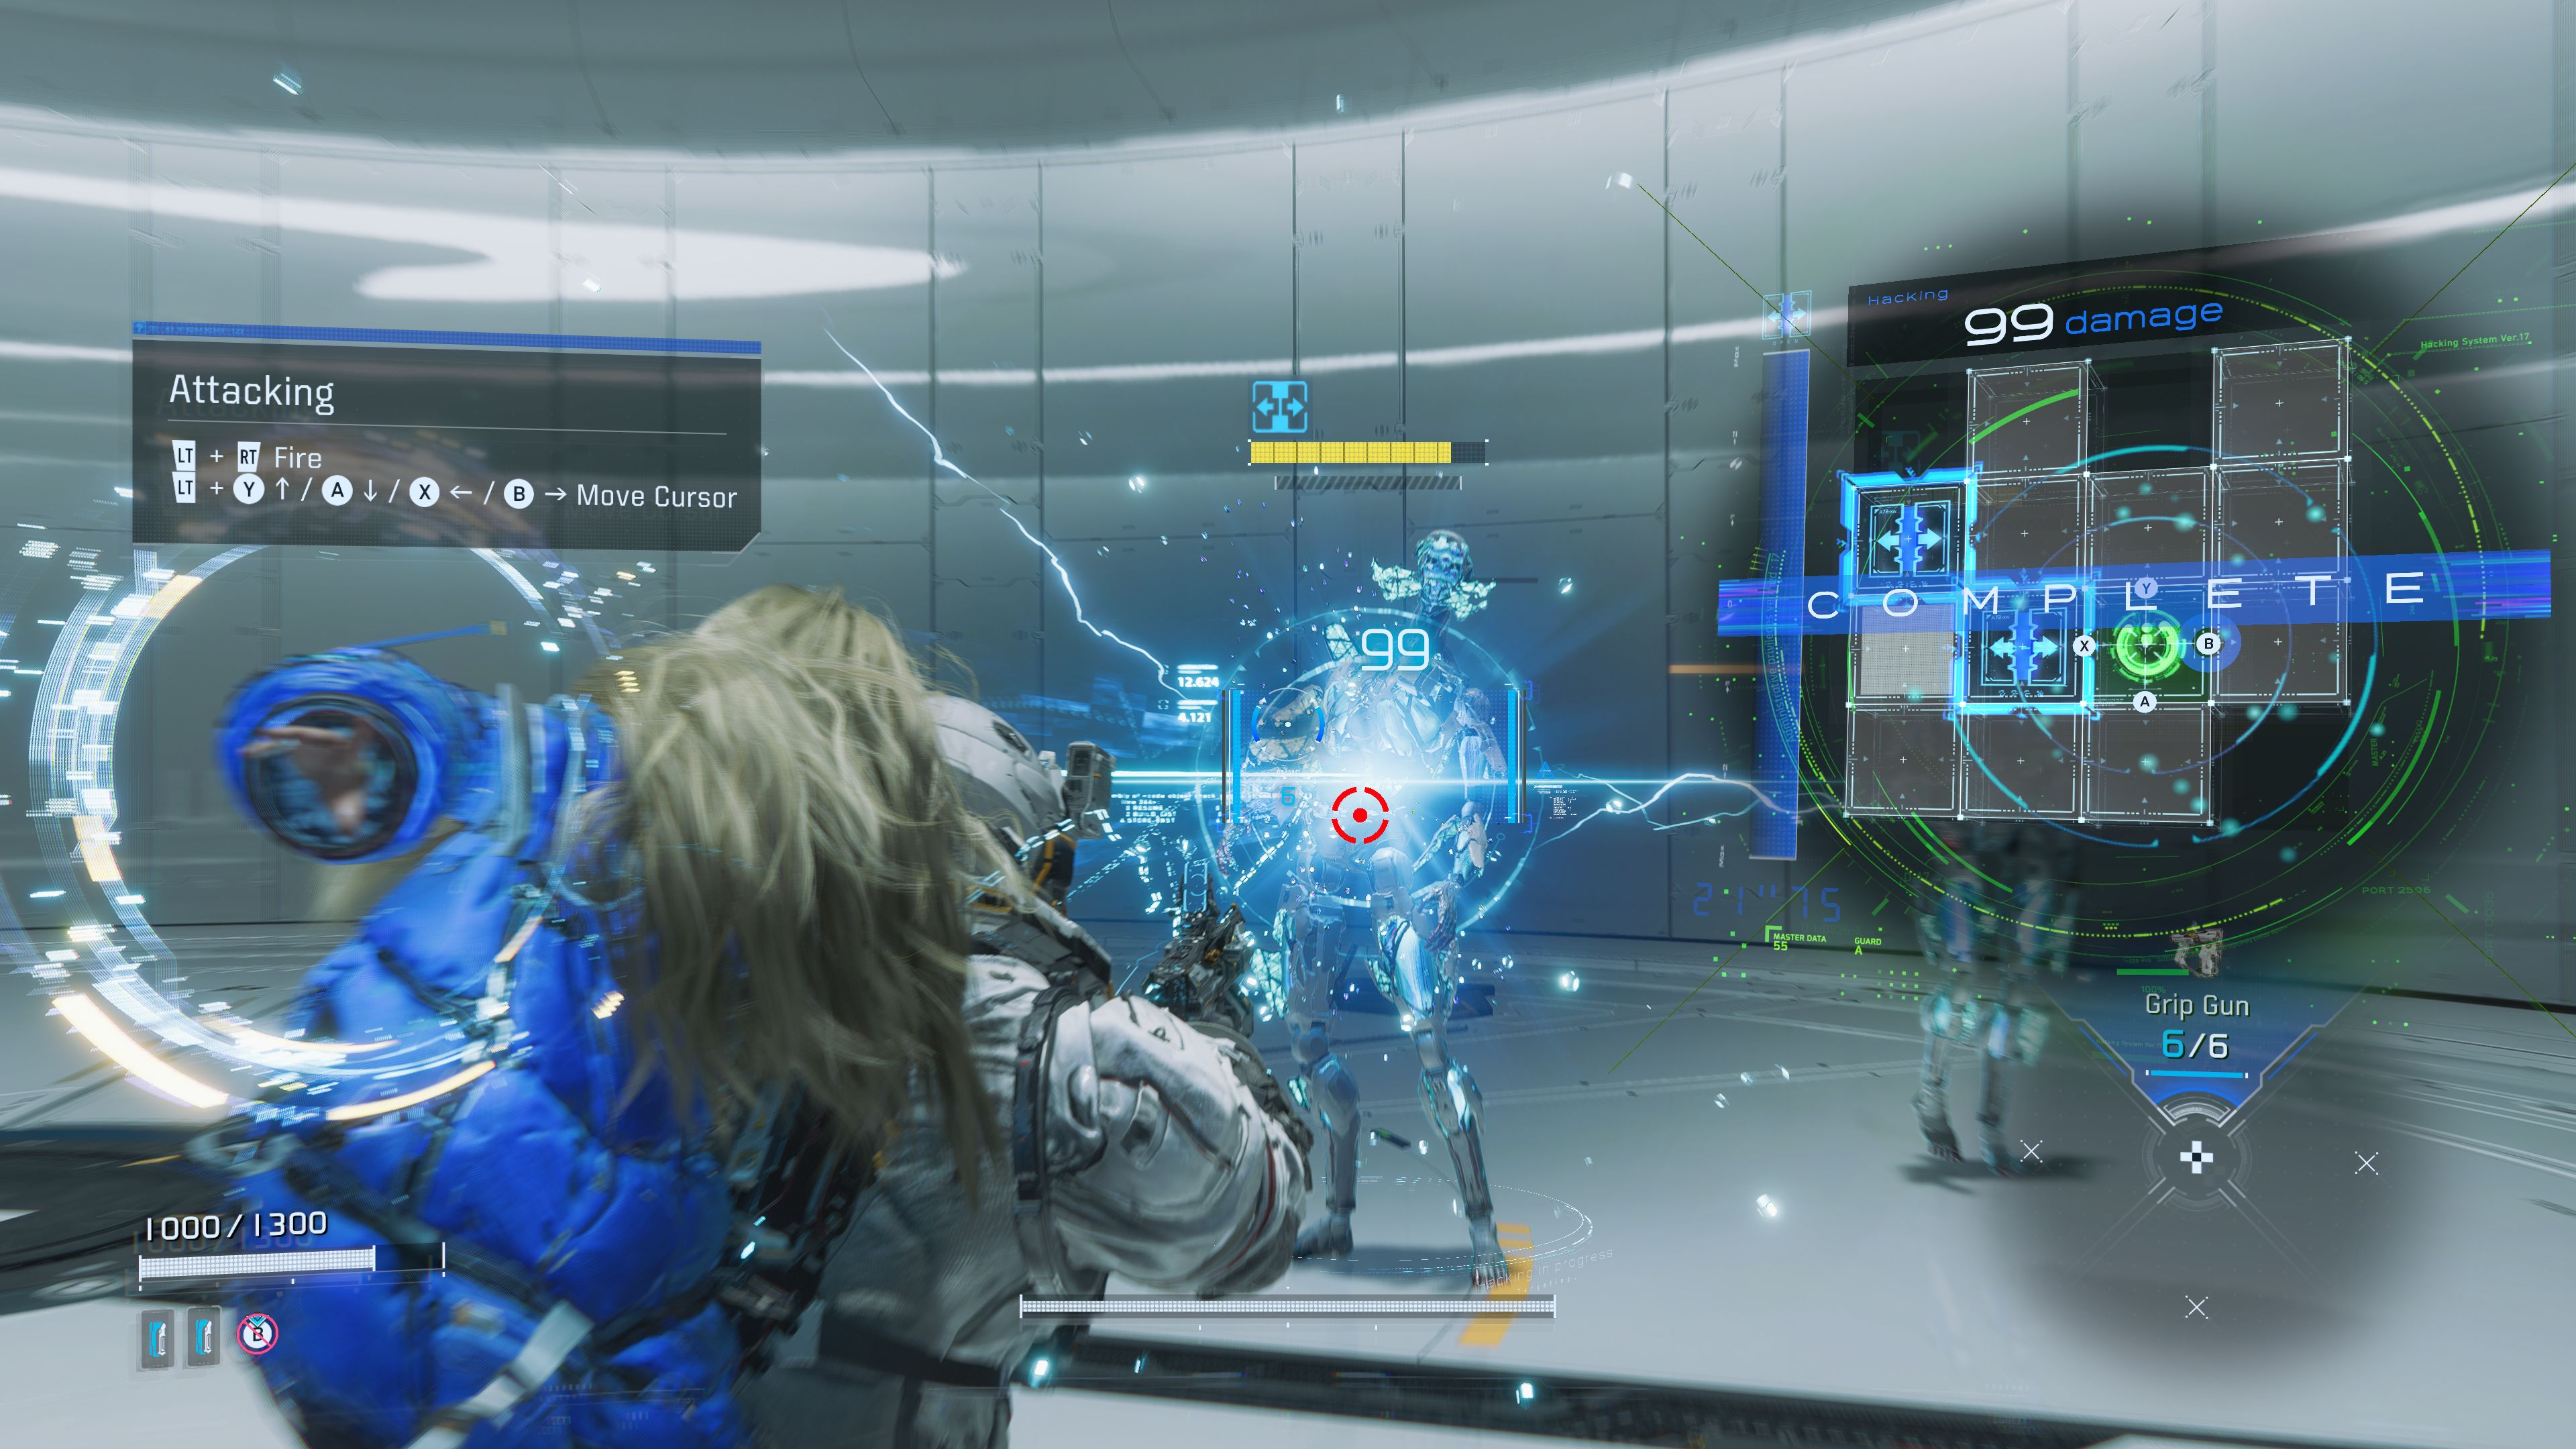
\includegraphics[width=\linewidth]{abbildungen/pragmata_screenshot}
        \caption{Finales Rendering einer Spielszene.}
        \label{fig:pragmata_final}
    \end{subfigure}

    \vspace{0.5cm} % Optionaler vertikaler Abstand zwischen den Teilabbildungen

    % Zweite Teilabbildung: G-Buffer / Render-Pässe
    \begin{subfigure}[b]{0.95\textwidth}
        \centering
        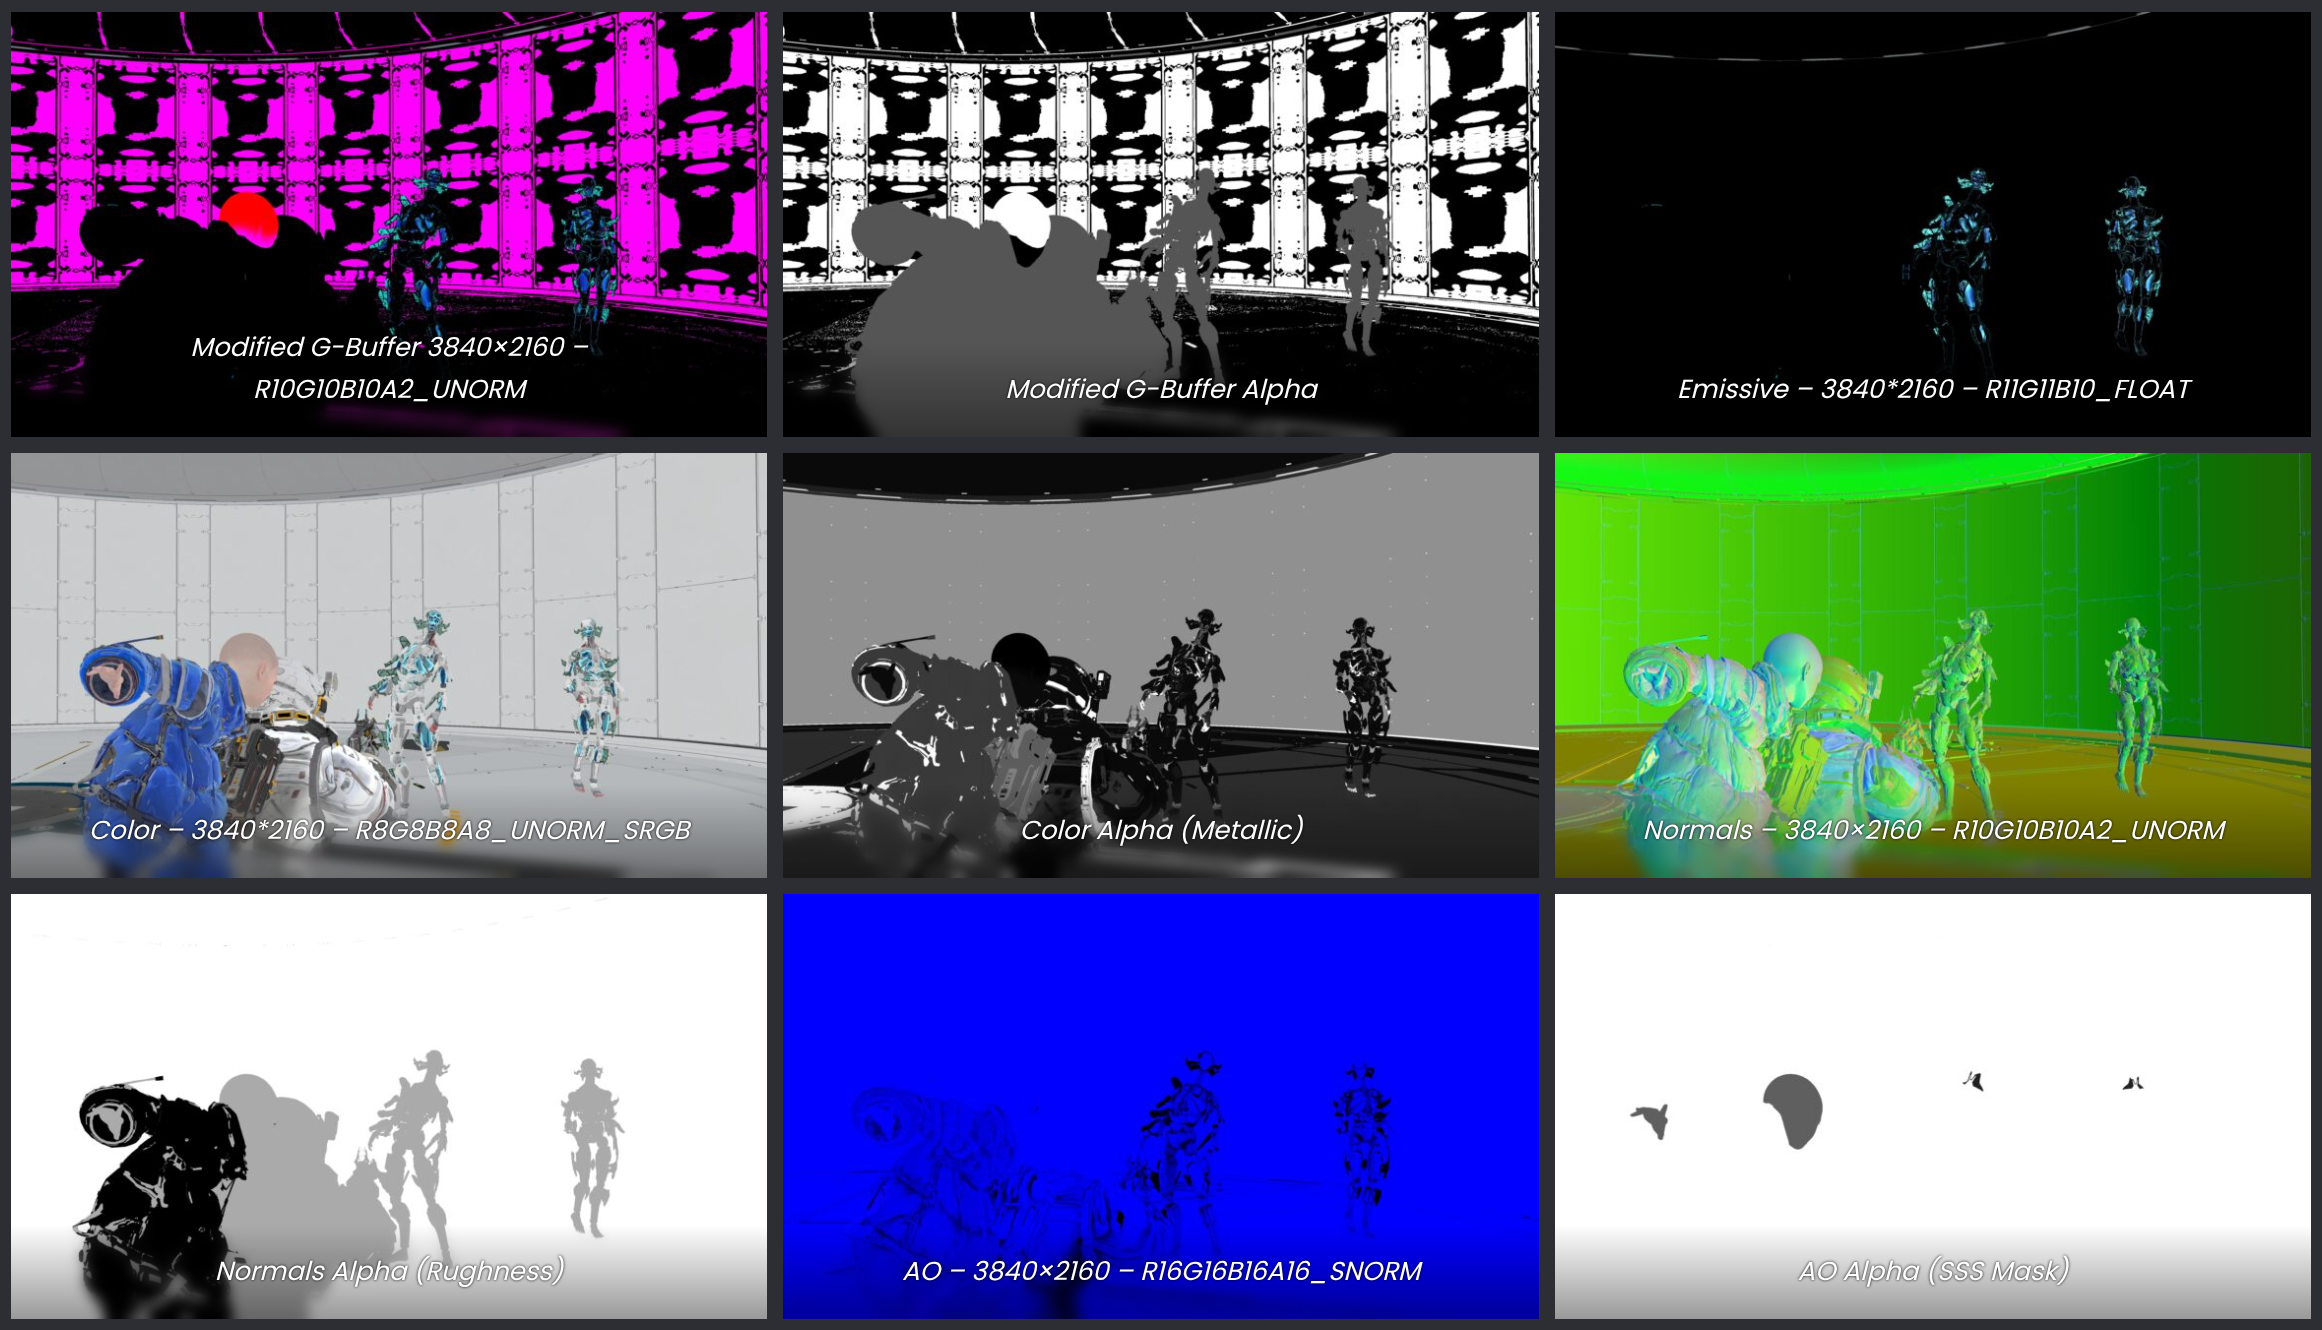
\includegraphics[width=\linewidth]{abbildungen/pragmata_gbuffer}
        \caption{Frame-Analyse des G-Buffers und der isolierten Render-Pässe.}
        \label{fig:pragmata_passes}
    \end{subfigure}

    % Gemeinsame Haupt-Caption
    \caption[Visualisierung der Pipeline-Fragmentierung in \textit{PRAGMATA}]{Visualisierung der Pipeline-Fragmentierung
    in modernen AAA-Produktionen am Beispiel von \textit{PRAGMATA} (2026) zur Veranschaulichung spezialisierter
    Industrie-Workarounds (Quelle: \cite{muhammadPrettyFramesPRAGMATA2026}).}
    \label{fig:pragmata_pipeline_analysis}
\end{figure}


\section{Limitierungen bestehender Ansätze und Identifikation der Forschungslücke}
\label{sec:0303_usp}

% Einleitung.
Wie in den Kapiteln~\ref{sec:0301_academic_state} und~\ref{sec:0302_industry_state} dargelegt, bieten sowohl die
Forschung als auch die Industriepraxis diverse, hochspezialisierte Lösungsansätze für architekturbedingte
Restriktionen klassischer Forward- und Deferred-Pipelines, ebenso im Kontext der selektiven Stilisierung
mittels \ac{NPR}.
Das Zusammenspiel dieser spezialisierten Optimierungen mit den grundlegenden Rendering-Paradigmen bleibt jedoch
weitgehend unbetrachtet.

% Forschungslücke.
Globale Screen-Space-Filter stellen in der Praxis einen einfachen und etablierten Standard
dar~\cite[S.~147]{magdicsPostprocessingNPREffects2013}.
Im spezifischen Kontext der selektiven, objektbasierten Stilisierung, vornehmlich innerhalb der weit verbreiteten
Deferred-Rendering-Paradigmen, stoßen gängige Praktiken jedoch in Abhängigkeit von der intendierten visuellen Stilistik
an grundlegende architektonische Grenzen.
Industrie-Workarounds wie Stencil-Maskierungen, dediziertes \ac{G-Buffer}-Packing oder der Einsatz hybrider Pipelines
versprechen hierbei zwar Abhilfe, erschweren jedoch durch ihre hohe Spezialisierung eine allgemeingültige Bewertung.
Aus Sicht der Entwicklungspraxis bleibt dadurch unklar, ab welcher Szenenkomplexität welche Lösung architektonisch zu
bevorzugen ist.

% Empirische Evidenz.
Theoretische Performance-Engpässe wie Bandbreitenlimitierungen im \ac{G-Buffer} oder hoher Registerdruck in
Uber-Shadern sind in der Literatur zwar
dokumentiert~\cites[S.~881]{akenine-mollerRealtimeRendering2019}[Abschn.~2.6]{Thaler2011DeferredRendering}
[Abschn.~6]{schiedDeferredAttributeInterpolation2015}.
Wie~\textcite[S.~905]{akenine-mollerRealtimeRendering2019} jedoch anmerken, verschieben sich diese Limitierungen in der
Praxis dynamisch mit der jeweiligen Szenenkomplexität.
Dies basiert auf einem Mangel an isolierten, komparativen Messdaten, welche das Skalierungsverhalten der
Basis-Paradigmen im \ac{NPR}-Kontext quantifizieren.

% Abgrenzung und Negative-Scope.
Da eine vollumfängliche Analyse sämtlicher industriespezifischer Workarounds den Untersuchungsumfang dieser Arbeit
überschreiten würde, erfordert die Gewährleistung valider empirischer Messungen eine strikte Limitierung des
Untersuchungsraums.
Komplexe Sondereffekte oder Optimierungen wie Transluzenzen, moderne Clustered-Techniken oder Anti-Aliasing-Ansätze
werden für diese fundamentale Basis-Analyse bewusst exkludiert.
Der Fokus liegt isoliert auf der Wechselwirkung zwischen opaker Geometrie, dynamischer Beleuchtung und materialbasierter
\ac{NPR}-Shader-Verarbeitung.

% Lösungsansatz und Legitimation der vorliegenden Arbeit.
Die Schließung dieser Forschungslücke erfordert ein isoliertes Messinstrument, das die
zugrundeliegenden Rendering-Architekturen anhand ihrer reinen Basis-Paradigmen und
frei von proprietärem Engine-Overhead evaluiert.
Das im Rahmen dieser Arbeit entwickelte Evaluations-Framework \ac{HyDra} bildet den zentralen Kern dieses Vorhabens
und dient dessen methodischer Umsetzung (siehe Abb.~\ref{fig:hydra_example}).
Die Evaluation der systematischen Verschiebung von Performance-Engpässen erfolgt über den Vergleich primärer
Rendering-Paradigmen: Single-Pass-Forward-Rendering, Single-Pass-Deferred-Rendering mit \ac{G-Buffer}-Packing über
\textit{Style-IDs} und Uber-Shader sowie Deferred-Rendering mit Light-Volumes als Referenz für Multi-Pass-Architekturen.
Durch die Erhebung granularer Rohdaten unter skalierender Stil-Entropie und Szenenkomplexität soll das in
Kapitel~\ref{sec:0102_goal_and_core_question} skizzierte heuristische Entscheidungsmodell abgeleitet werden.
Die technische Konzeption sowie die architektonischen Spezifika dieses Frameworks bilden den Schwerpunkt des
nachfolgenden Kapitels.

\begin{figure}[htbp]
    \centering
    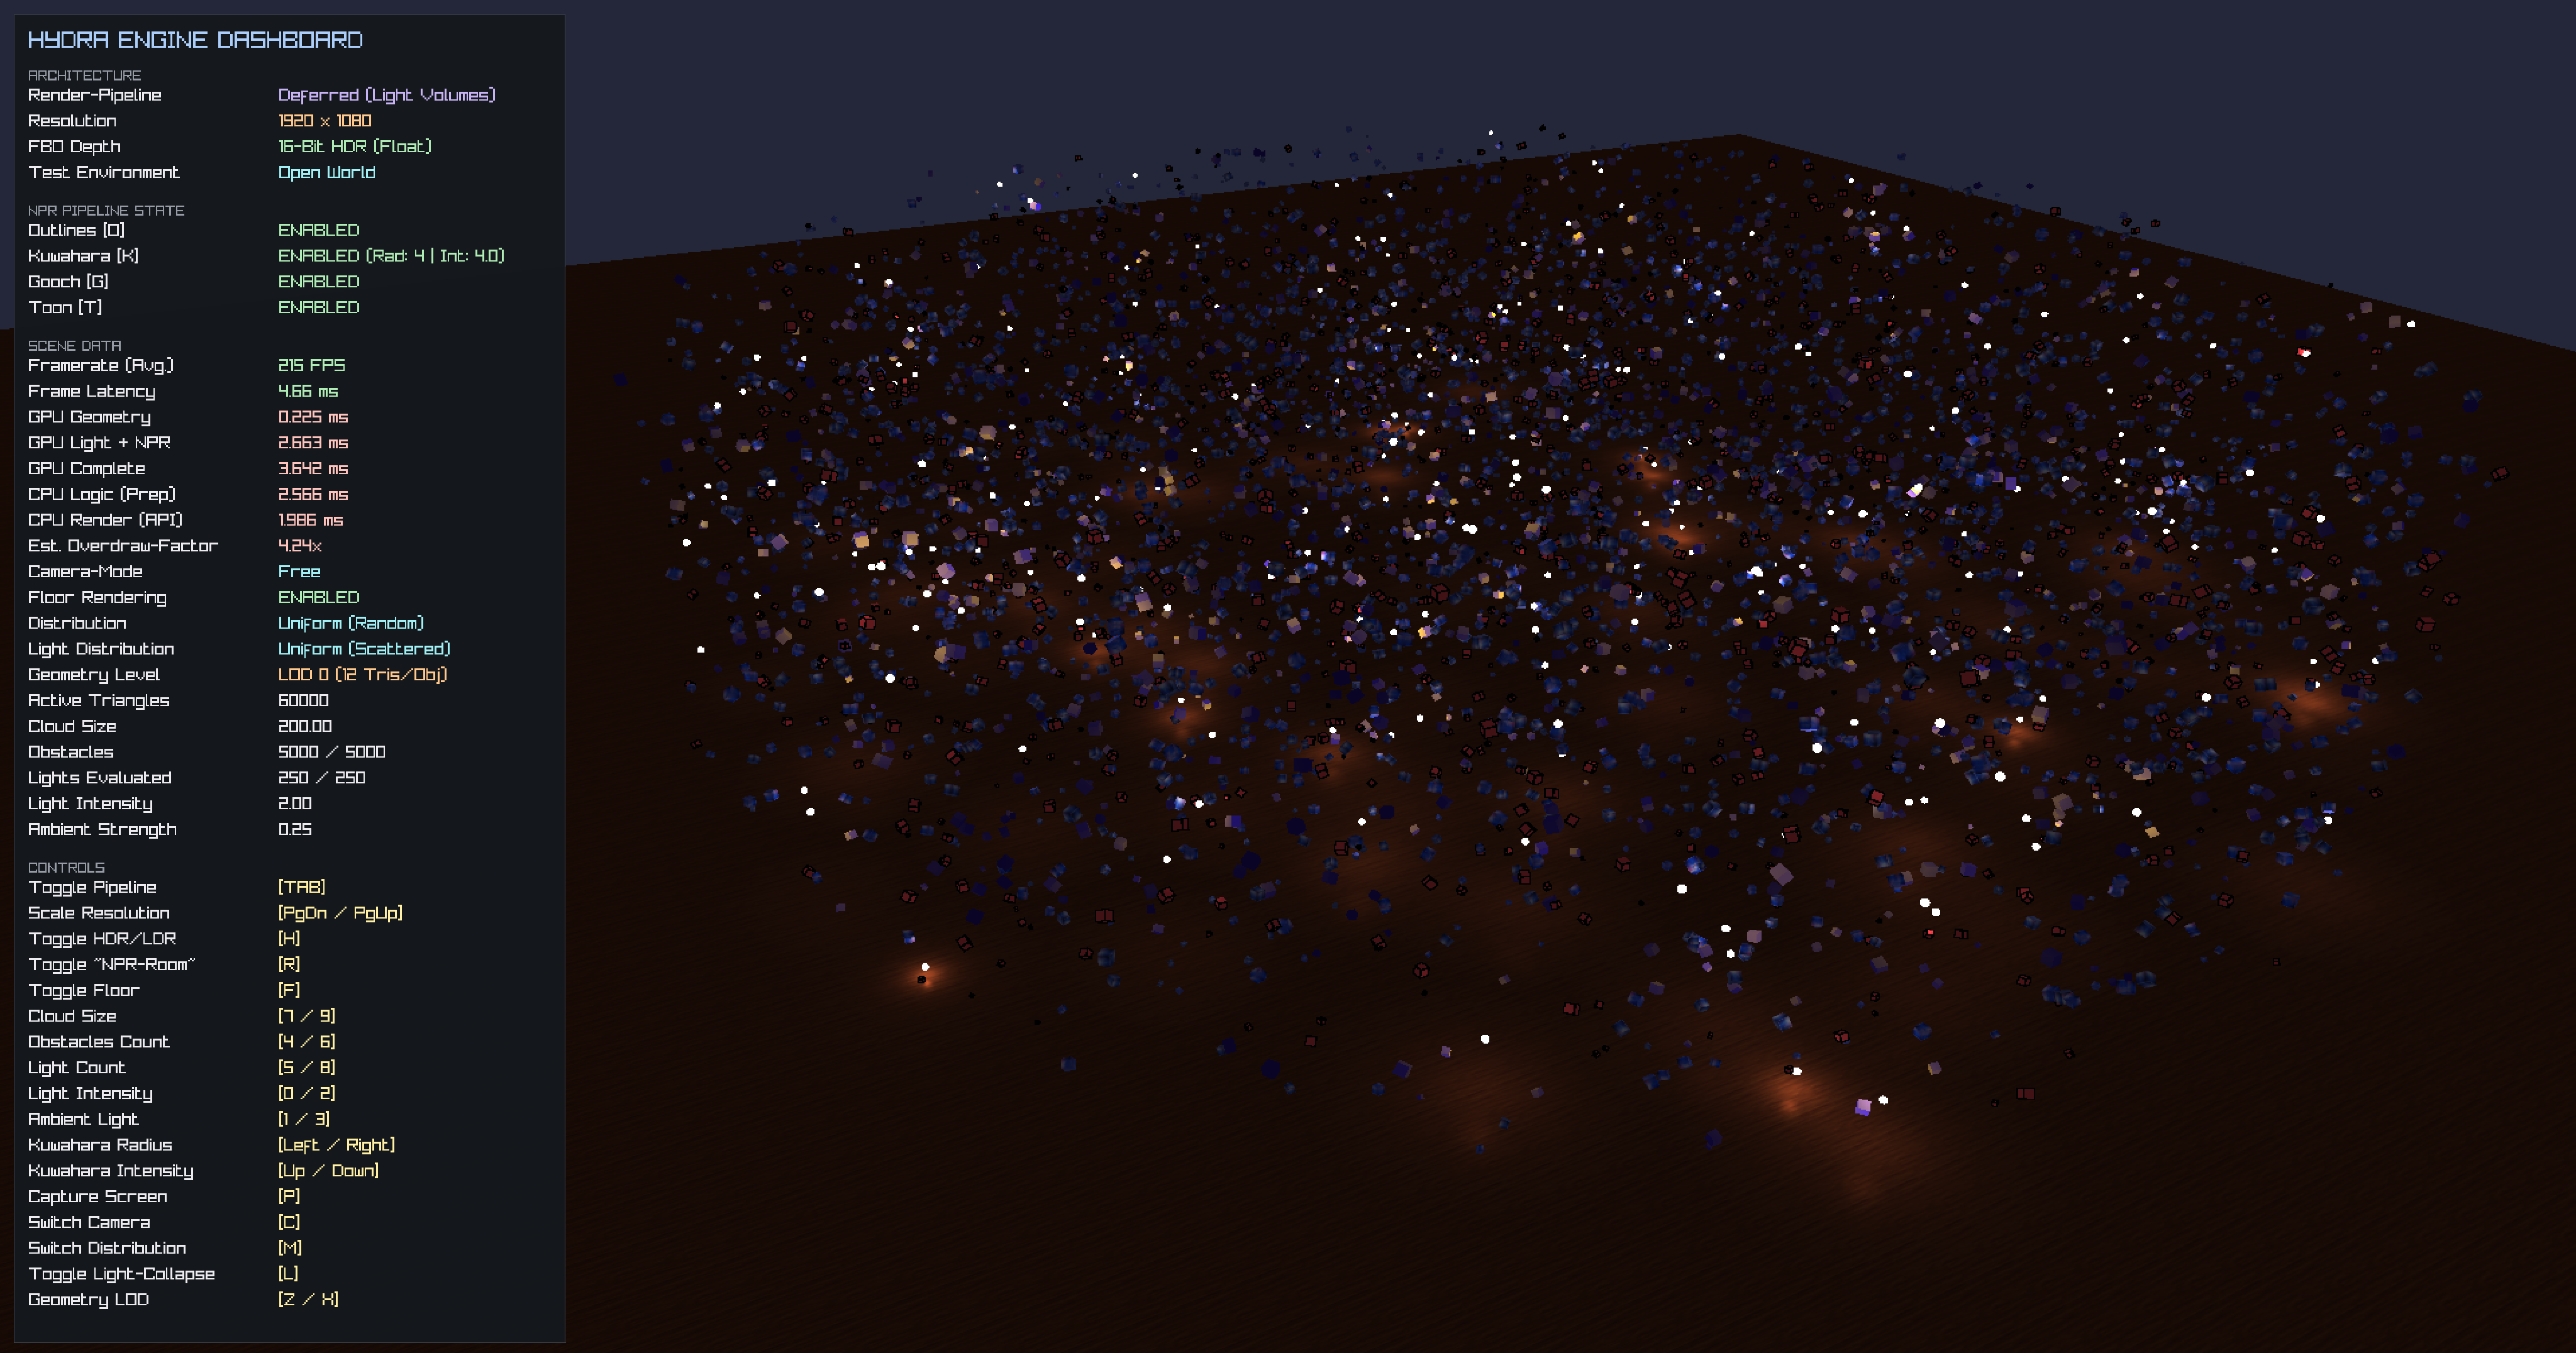
\includegraphics[width=0.95\linewidth]{abbildungen/hydra_capture_20260717_200713}
    \caption[Screenshot aus dem HyDra-Framework]{Screenshot aus dem HyDra-Framework.}
    \label{fig:hydra_example}
\end{figure}


